\apendice{Plan de Proyecto Software}

\section{Introducción}

En este apartado se expone como se ha planteado el proyecto a lo largo del tiempo, y su viabilidad tanto económica como legal. 
\section{Planificación temporal}
Para la planificación temporal, cabe destacar que se ha seguido la metodología SCRUM, la cual no se ha podido seguir al 100\%, puesto que es una metodología planeada para equipos de trabajo, siendo este un proyecto personal de final de carrera. 

\begin{itemize}
    \item Se programó el \textit{sprint} de dos semanas, donde, se podrían haber hecho de una semana, pero la metodología SCRUM recomienda de dos a cuatro.
    \item Durante, el  \textit{sprint} se planean unas tareas a terminar en el periodo de tiempo.
    \item Cada tarea tiene un objetivo y una estimación; se organizan en un tablero canvas con las siguientes columnas consideradas:
    \begin{itemize}
        \item ``tareas a realizar'' : Son las tareas planeadas para el sprint actual o próximos.
        \item ``tareas en proceso'' : Son aquellas tareas que se están realizando en el momento.
        \item ``tareas terminadas'' : Son las tareas que ya se han terminado, las cuales se comprueban al final del sprint si se han terminado correctamente, en tal caso se cierran.
        \item ``tareas cerradas'' : Son aquellas tareas que se han cerrado en \textit{sprints} anteriores, las cuales se han implementado correctamente en el producto final. 
    \end{itemize}
    \item Con los gráficos \textit{burndown}, se puede observar el proceso del proyecto de cada \textit{sprint}
    \item Como se ha comentado, al terminar el sprint, se realizaba una reunión personal, donde se comprobaba si se habían completado correctamente las tareas terminadas. En caso de no ser así, se añadía para el siguiente \textit{sprint}, además, se añadían las nuevas tareas a realizar en el siguiente.
\end{itemize}
Esta metodología se ha implementado usando la herramienta ZenHub, la cual permite hacer los apartados anteriores con facilidad.
Para asignar los pesos de la tarea, se utiliza una aproximación de la secuencia de fibonacci. Donde los valores dependen del tiempo y dificultad que llevará la tarea, esta estimación, a lo largo del proyecto va siendo más precisa, puesto que, al principio, no se controlaban los tiempos que conllevarían las dificultades del proyecto.

Los \textit{sprints} que se realizaron se comentan a continuación.

\subsection{Sprint 0 - Anterior al 27/12/2022}
En este sprint inicial, del que no se poseen fechas, se realizaron diversas reuniones, en las cuales se explicaron en que iba a consistir el proyecto.

Durante este sprint, se estuvo investigando sobre aplicaciones Android con el mismo objetivo, sobre las que basar el proyecto. Encontrando de esta forma la aplicación Ret-iN CaM. La cual sirve para realizar estudios sobre los pacientes, de forma que se pueda ver la evolución.
Además, se realizaron búsquedas sobre redes neuronales ya creadas las cuales añadir a la aplicación. 

Como este sprint fue más un periodo de búsqueda de información, sin realizar ningún trabajo real, no se contabilizó el trabajo realizado.
\subsection{Sprint 1 - 27/12/2022 - 10/01/2023}
En este primer Sprint, se estuvo pensando con que herramienta realizar el proyecto. Teniendo como objetivo crear tanto el proyecto, como el LaTeX.

Para la aplicación móvil, se pensaba utilizar o Android Studio o Unity, de Android Studio ya se tenían conocimientos de uso, pero de Unity no, por ello, se realizó un proyecto ''Hola Mundo'' en Unity, para ver la complejidad; al ver que la herramienta estaba más destinada a aplicaciones gráficas, se decidió realizar la aplicación en Android Studio, creando el proyecto.

Para la realización del documento, se pensó hacer de forma local, utilizando MiKTeX, pero por facilidad de uso de los tutores, quienes preferían el uso de OverLeaf, que les permitía corregir de forma concurrente el documento, se utilizó esta.

Como este primer sprint se estaba empezando, y además era Navidad, se olvidó mover las tareas de ZenHub a terminadas, y la gráfica que proporciona ZenHub es incorrecta. Se puede ver en \ref{fig:Sprint1}

\begin{figure}[!ht]
         \centering
         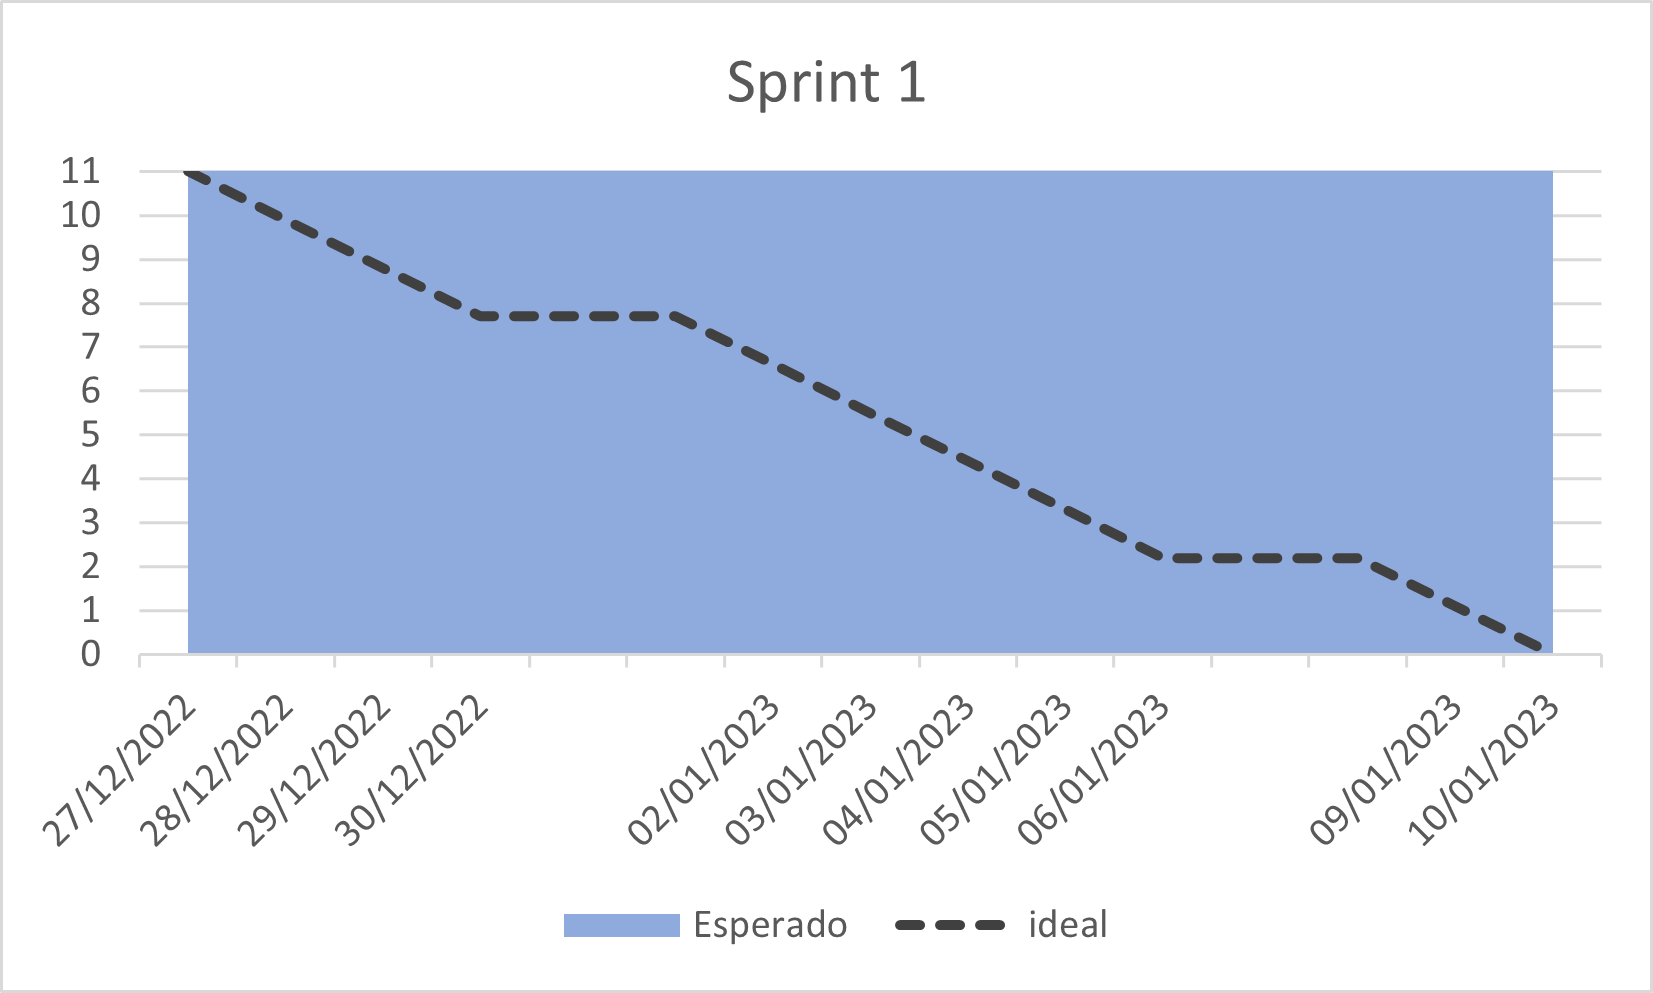
\includegraphics[width=0.9\textwidth]{burndown/primerSprint.png}
         \caption{Sprint 1}
         \label{fig:Sprint1}
\end{figure}

\subsection{Sprint 2 - 10/01/2023 - 24/01/2023}
En el segundo Sprint se planeó hacer el menú principal de la aplicación, para ir haciendo la interfaz de usuario y a su vez, se hizo una investigación sobre que colores relaciona el ser humano con la retinopatía diabética.
Para hacer el menú, primero se hizo un boceto a mano, por ese motivo, se puso un valor alto de la estimación.
Por otro lado, se investigó sobre como implementar las redes neuronales en Android Studio, e ir añadiendo apartados al documento LaTeX.

De estas tareas, no se pudieron terminar ni la de investigar como implementar una red neuronal en Android Studio, ni añadir el apartado en concreto del LaTeX. Aunque si que se avanzó, SCRUM no permite dividir la tarea en parte terminada y parte que no, por lo que se va a considerar que no se han realizado.

El gráfico burndown se vería incorrectamente, debido al inconveniente ocurrido en el primer sprint, arreglando este defecto, se vería en la imagen~\ref{fig:Sprint2}.

\begin{figure}[!ht]
         \centering
         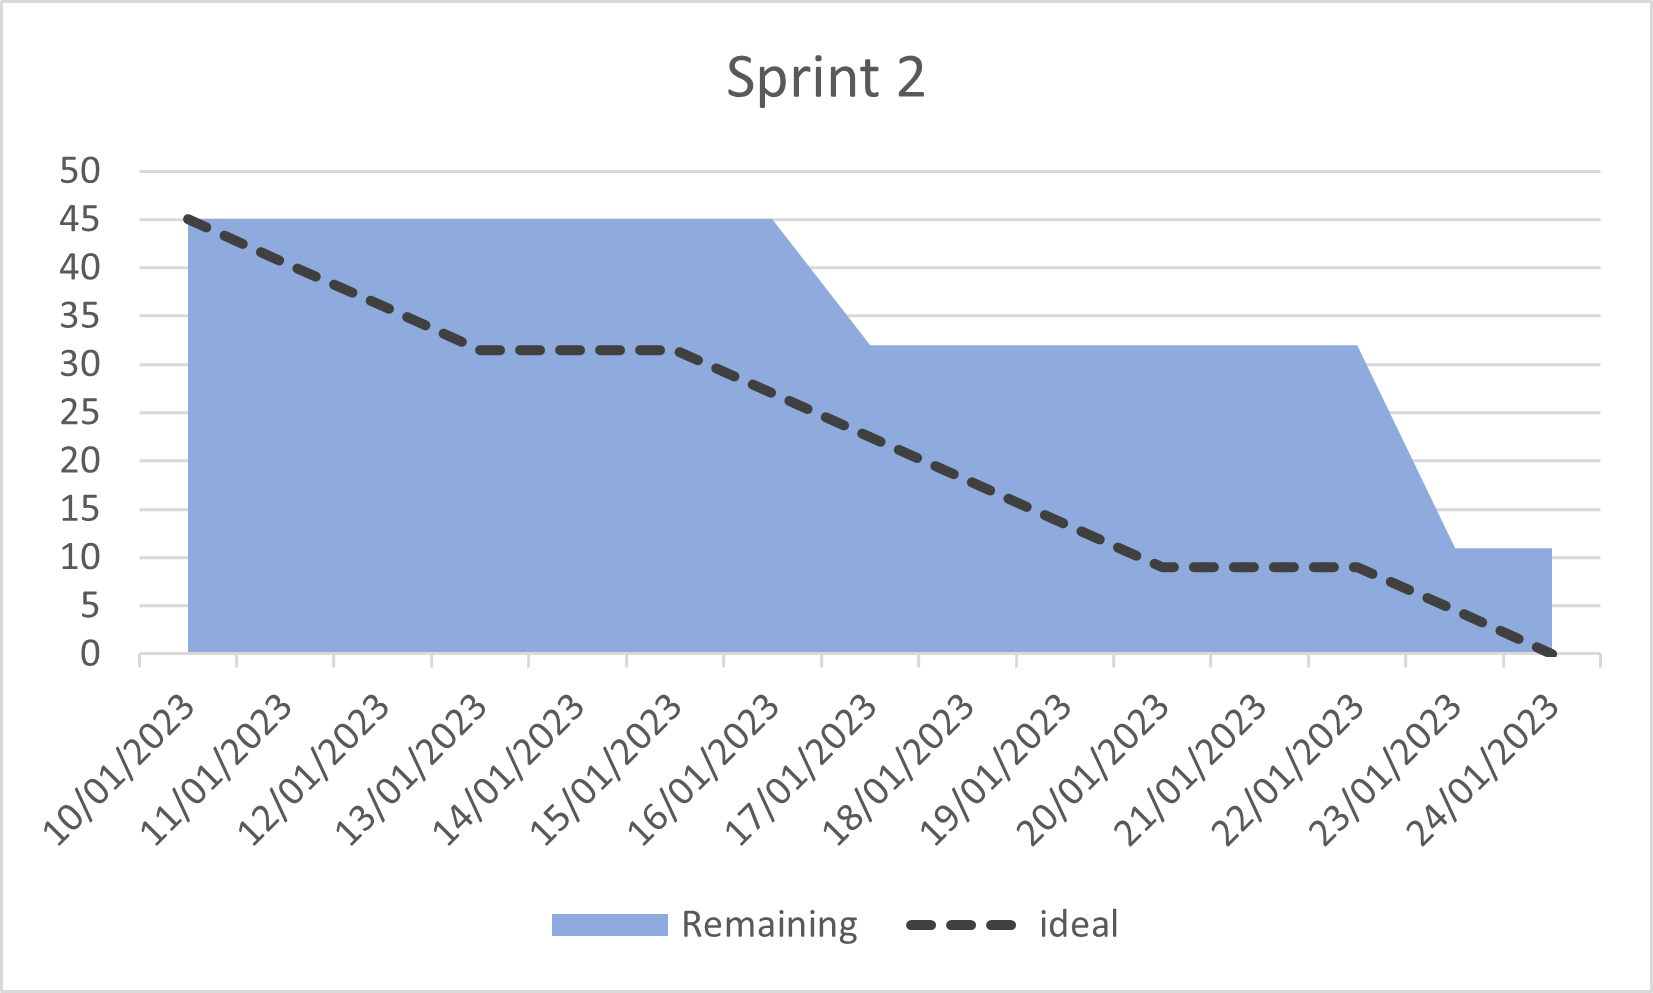
\includegraphics[width=0.9\textwidth]{burndown/segundoSprint.png}
         \caption{Sprint 2}
         \label{fig:Sprint2}
\end{figure}

\subsection{Sprint 3 - 24/01/2023 - 07/02/2023}
En el tercer Sprint, se añadieron las tareas no terminadas en el anterior, y se añadió también, el terminar el boceto inicial de la aplicación.
Al iniciar el sprint, se pensó en que la aplicación tenía que tener nombre y un logo, pero se programó para futuros sprints porque ya se tenían varias tareas para este.
Además, no se pudo avanzar mucho en la introducción del LaTeX porque era necesario aclarar una duda presencialmente, y la reunión se hizo a finales del sprint.

Como se iba avanzando en las tareas simultáneamente, tanto terminar el boceto de la aplicación y buscar información de la implementación, se terminaron el mismo día. \ref{fig:Sprint3}

\begin{figure}[!ht]
         \centering
         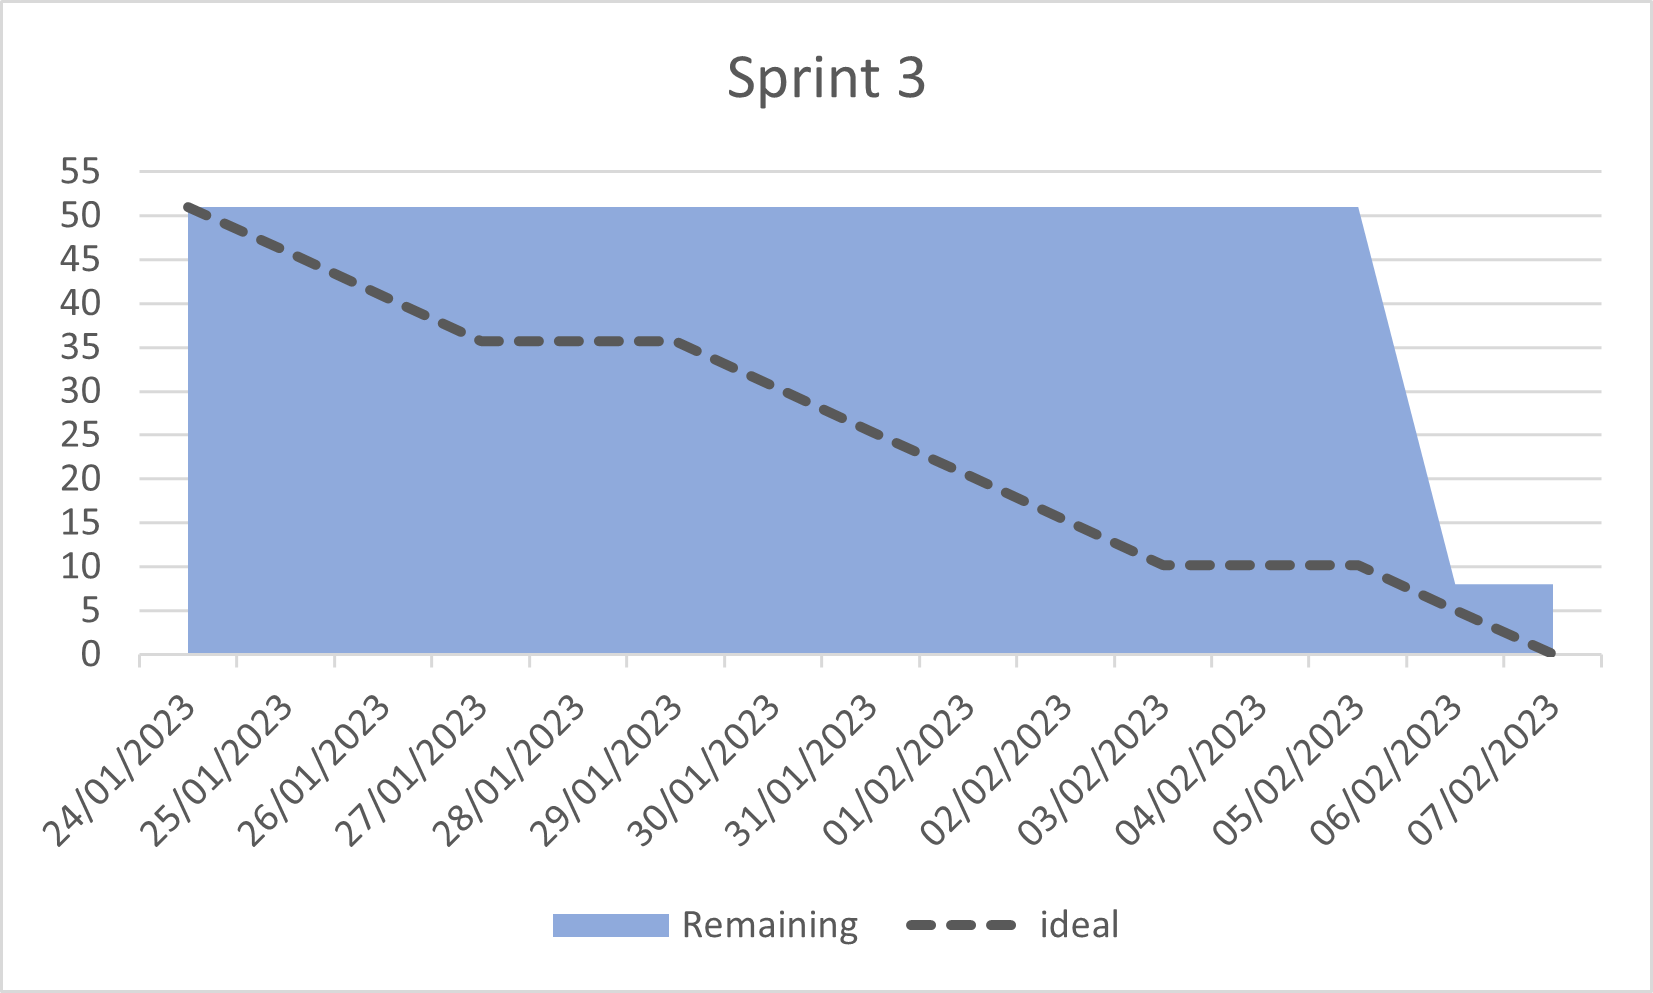
\includegraphics[width=0.9\textwidth]{burndown/tercerSprint.png}
         \caption{Sprint 3}
         \label{fig:Sprint3}
\end{figure}
\subsection{Sprint 4 - 07/02/2023 - 21/02/2023}
Para el cuarto sprint, se planeó realizar como una investigación sobre cómo se podría incluir la aplicación en la Play Store, y sobre como integrar Tensorflow en Android Studio.

Al investigar sobre la Play Store, se dio cuenta que era necesario realizar un pago de 25\$, por ese mismo motivo, se preguntó a los tutores, quienes dijeron que no hacía falta subir la aplicación a ninguna tienda.

Por otro lado, se terminaron las demás tareas, cumpliendo los objetivos del sprint. Y aunque se podría haber eliminado la tarea de investigación de la Play Store, el tiempo gastado en la investigación se había realizado, por lo que no se eliminó.

El burndown quedaría como indica la figura \ref{fig:Sprint4}. 
\begin{figure}[!ht]
         \centering
         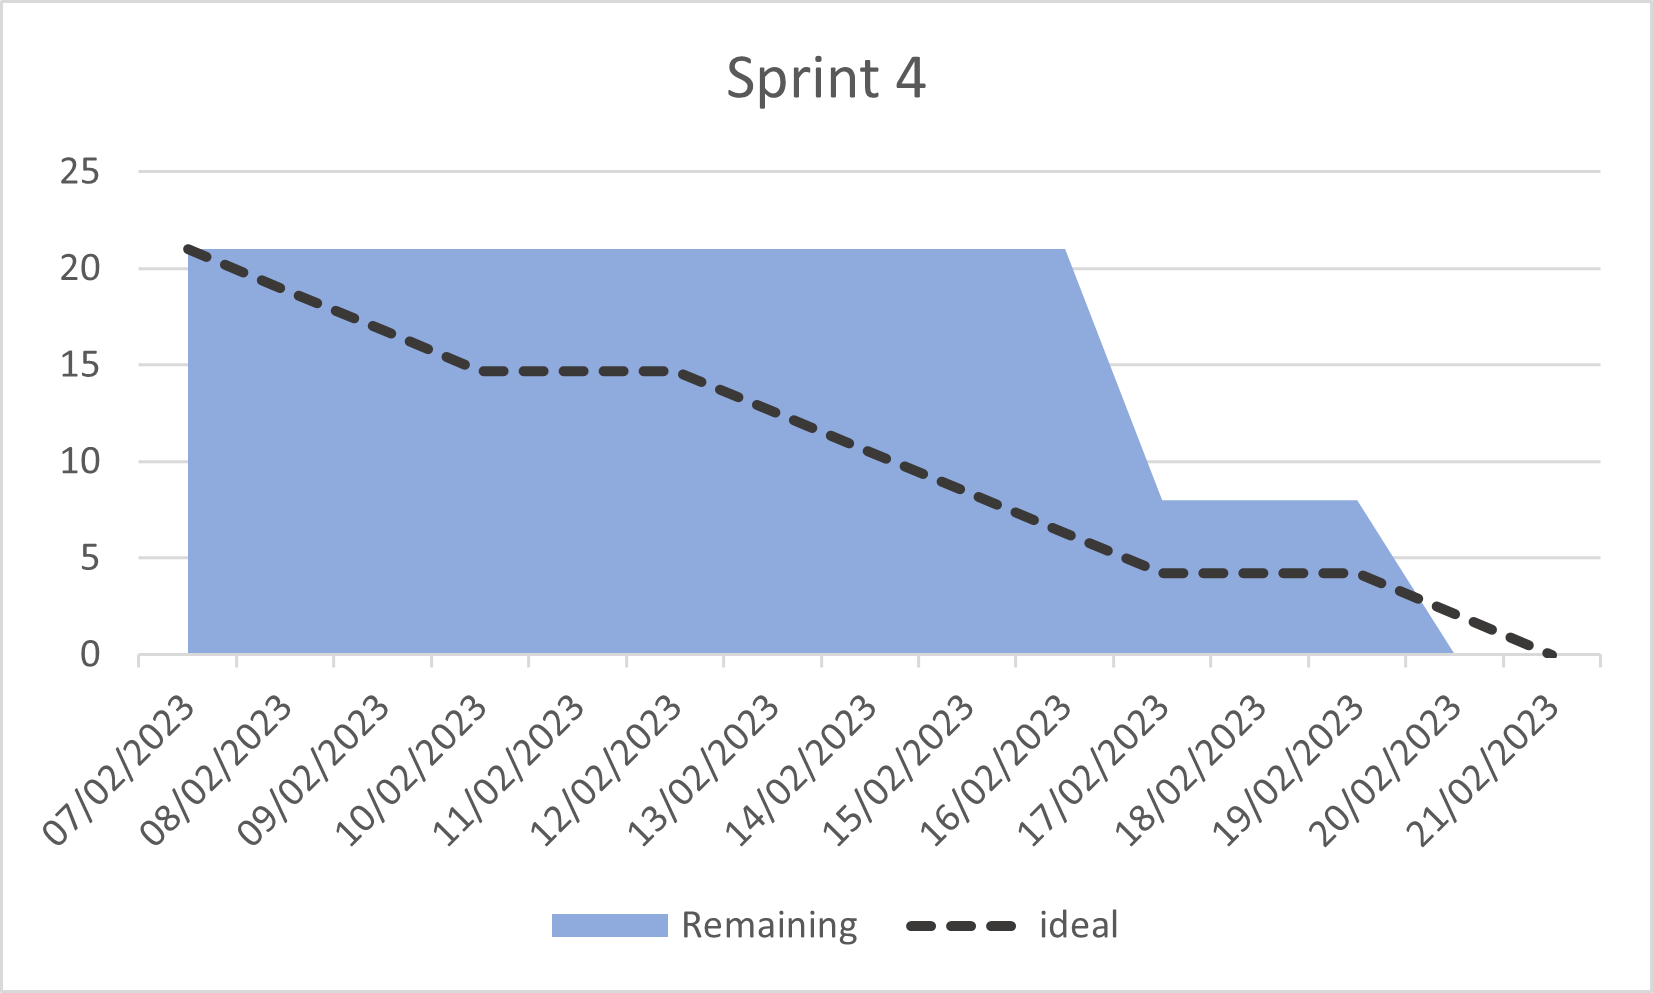
\includegraphics[width=0.9\textwidth]{burndown/cuartoSprint.png}
         \caption{Sprint 4}
         \label{fig:Sprint4}
\end{figure}


\subsection{Sprint 5 - 21/02/2023 - 07/03/2023}
Para este sprint, como no había tareas atrasadas, se añadieron la creación del logo y el nombre de la aplicación, de la investigación anterior de como implementar una red neuronal en Android Studio, el caso concreto de una red neuronal .h5; realizar cambios en la interfaz para añadir y quitar funcionalidad. Y añadir una base de datos; para lo que se pensó realizar un conjunto de clases java, las cuales simulaban la base de datos, y con un constructor, inicializar los datos.

Debido a que no se me da muy bien en el diseño artístico, se me ocurrió la idea de utilizar la herramienta DALL·E2 para un diseño preliminar, una vez se proporcionó un resultado aceptable, se editó el icono eliminando ruido, y cambiando los colores.

Debido a las diversas actividades designadas en este sprint, no se pudo realizar la base de datos.

Obteniendo el burndown \ref{fig:Sprint5}
\begin{figure}[!ht]
         \centering
         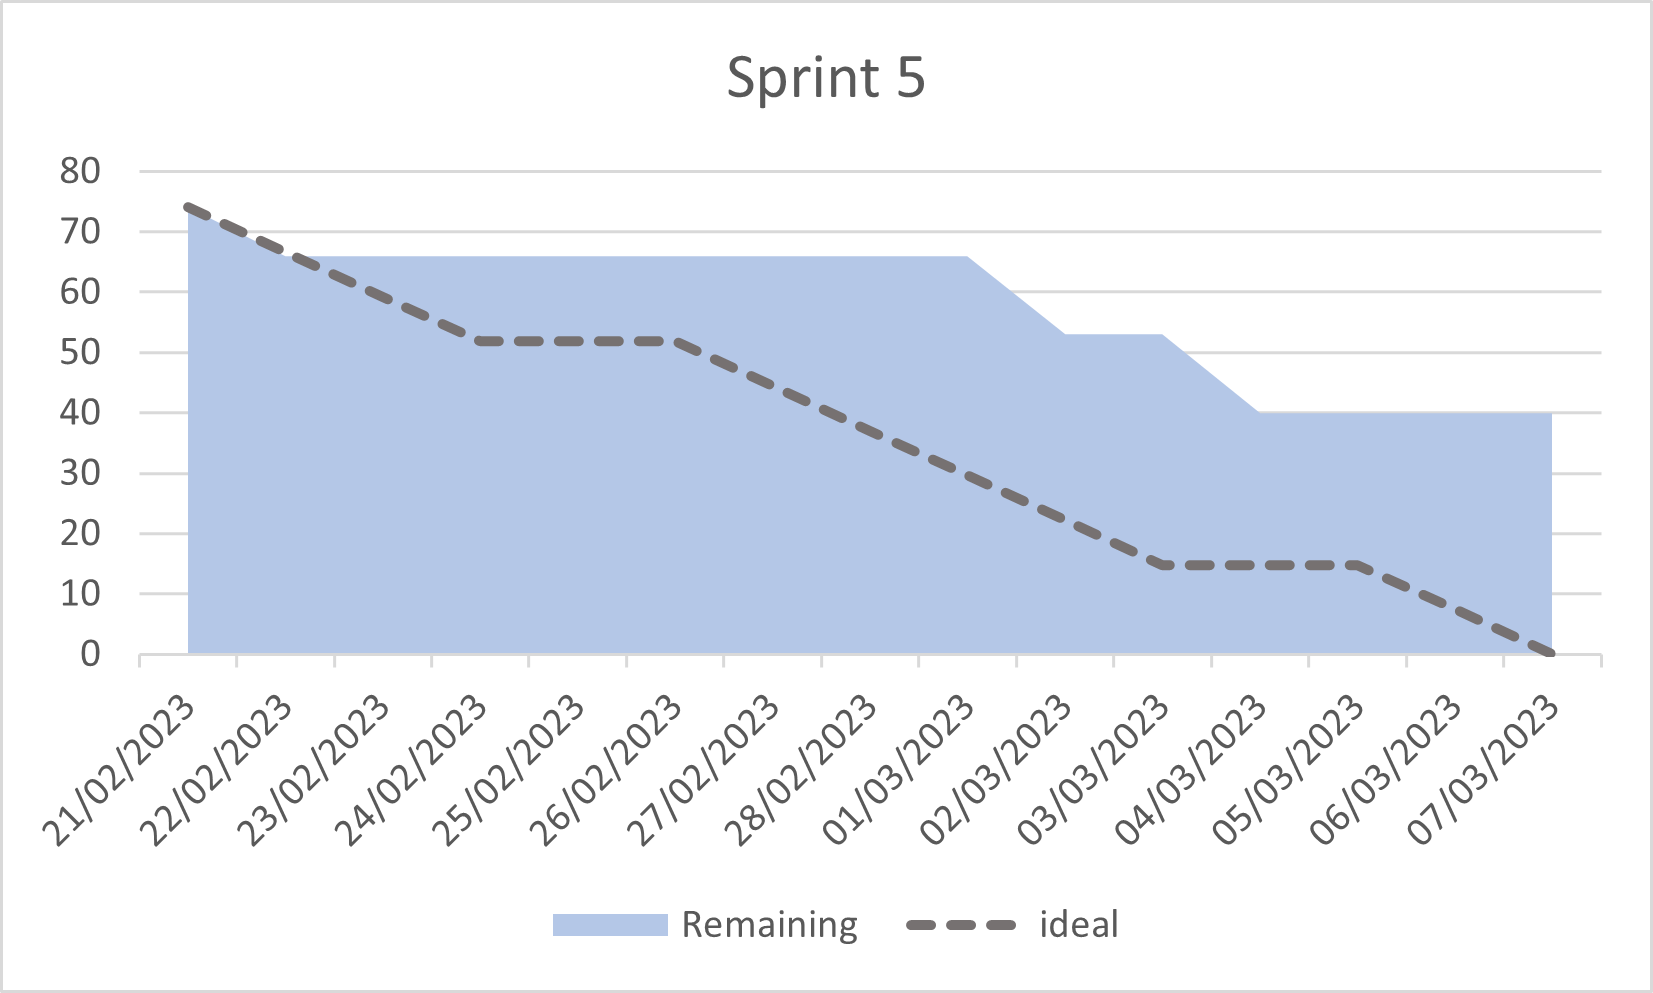
\includegraphics[width=0.9\textwidth]{burndown/quintoSprint.png}
         \caption{Sprint 5}
         \label{fig:Sprint5}
\end{figure}
\subsection{Sprint 6 - 07/03/2023 - 21/03/2023}
En el sexto sprint, se añadieron realizar el apartado de trabajos relacionados del documento LaTeX, y probar una integración de una red neuronal básica.
Ambas tareas se terminaron, y se avanzó en la creación de la base de datos; pero no se terminó debido a que se querían añadir más datos, los cuales solo se crearon un médico, un paciente y un informe.

Sin contar que se podría haber considerado como la tarea terminada, el gráfico burndown, sería \ref{fig:Sprint6}.
\begin{figure}[!ht]
         \centering
         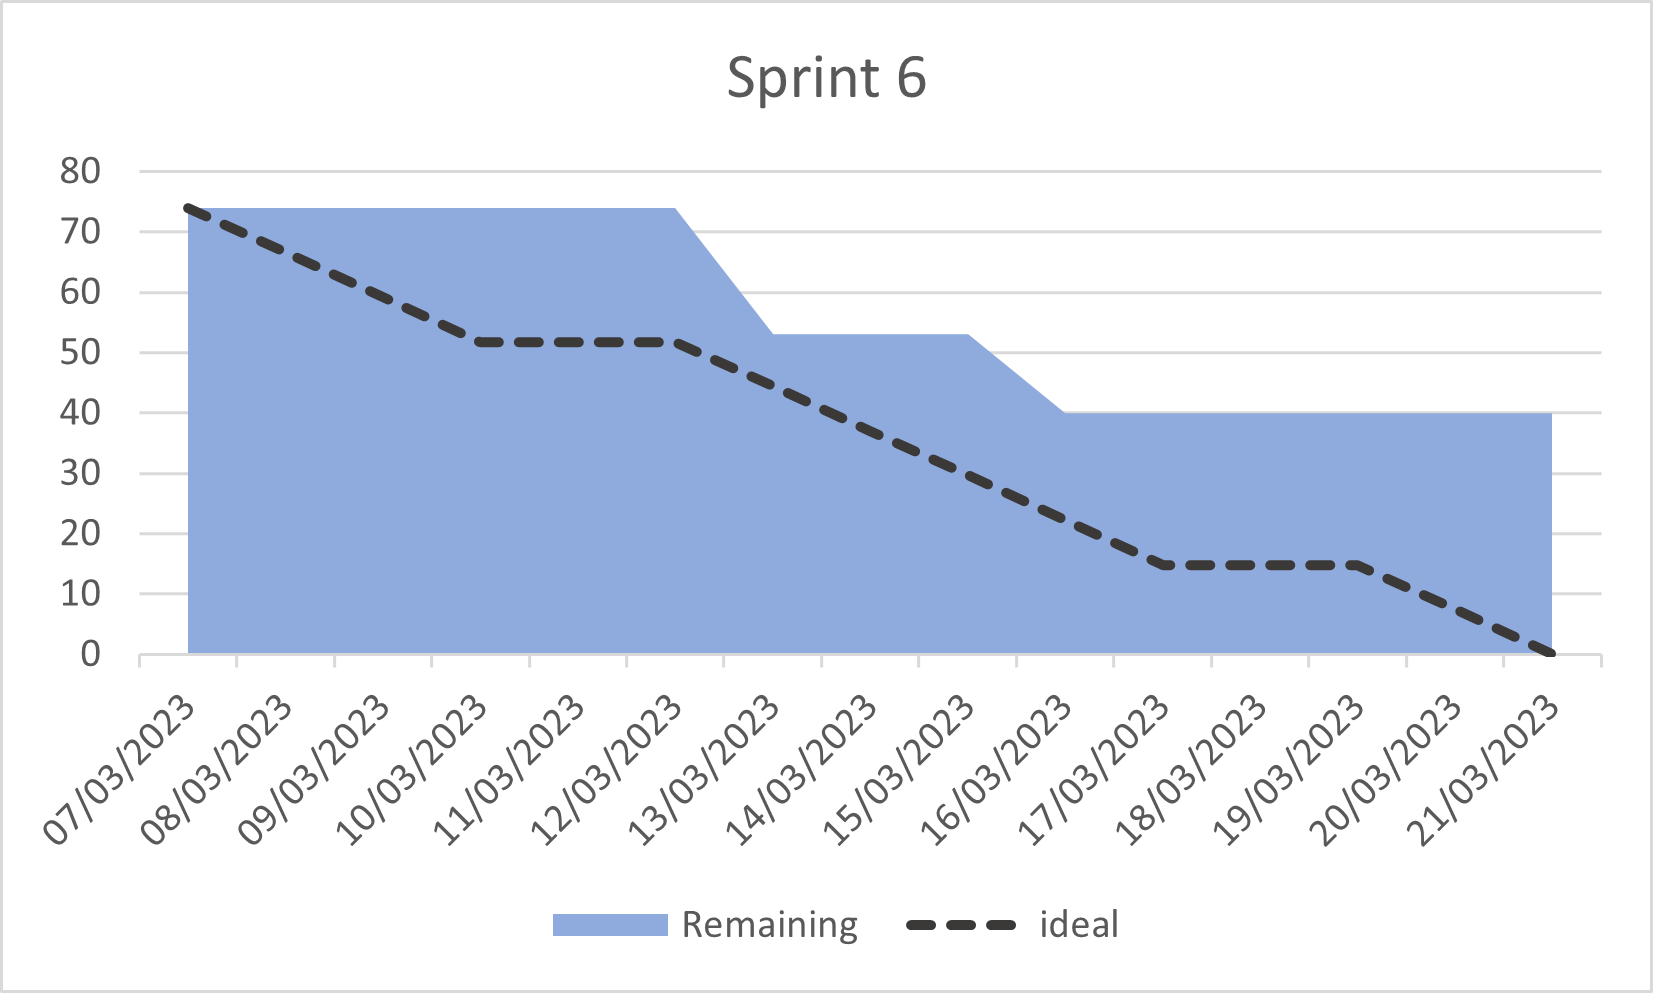
\includegraphics[width=0.9\textwidth]{burndown/sextoSprint.png}
         \caption{Sprint 6}
         \label{fig:Sprint6}
\end{figure}

\subsection{Sprint 7 - 21/03/2023 - 04/04/2023}
En este sprint, se terminó la base de datos añadiendo otro par de pacientes y médicos, y se planearon hacer una eliminación de bugs, debido al modo oscuro, y que no guardaba bien datos entre las distintas actividades. Y también se pensó hacer el apartado ``añadir técnicas y herramientas'', pero se avanzó, sin poder acabar la tarea. Quedando para el siguiente sprint.
\ref{fig:Sprint7}
\begin{figure}[!ht]
         \centering
         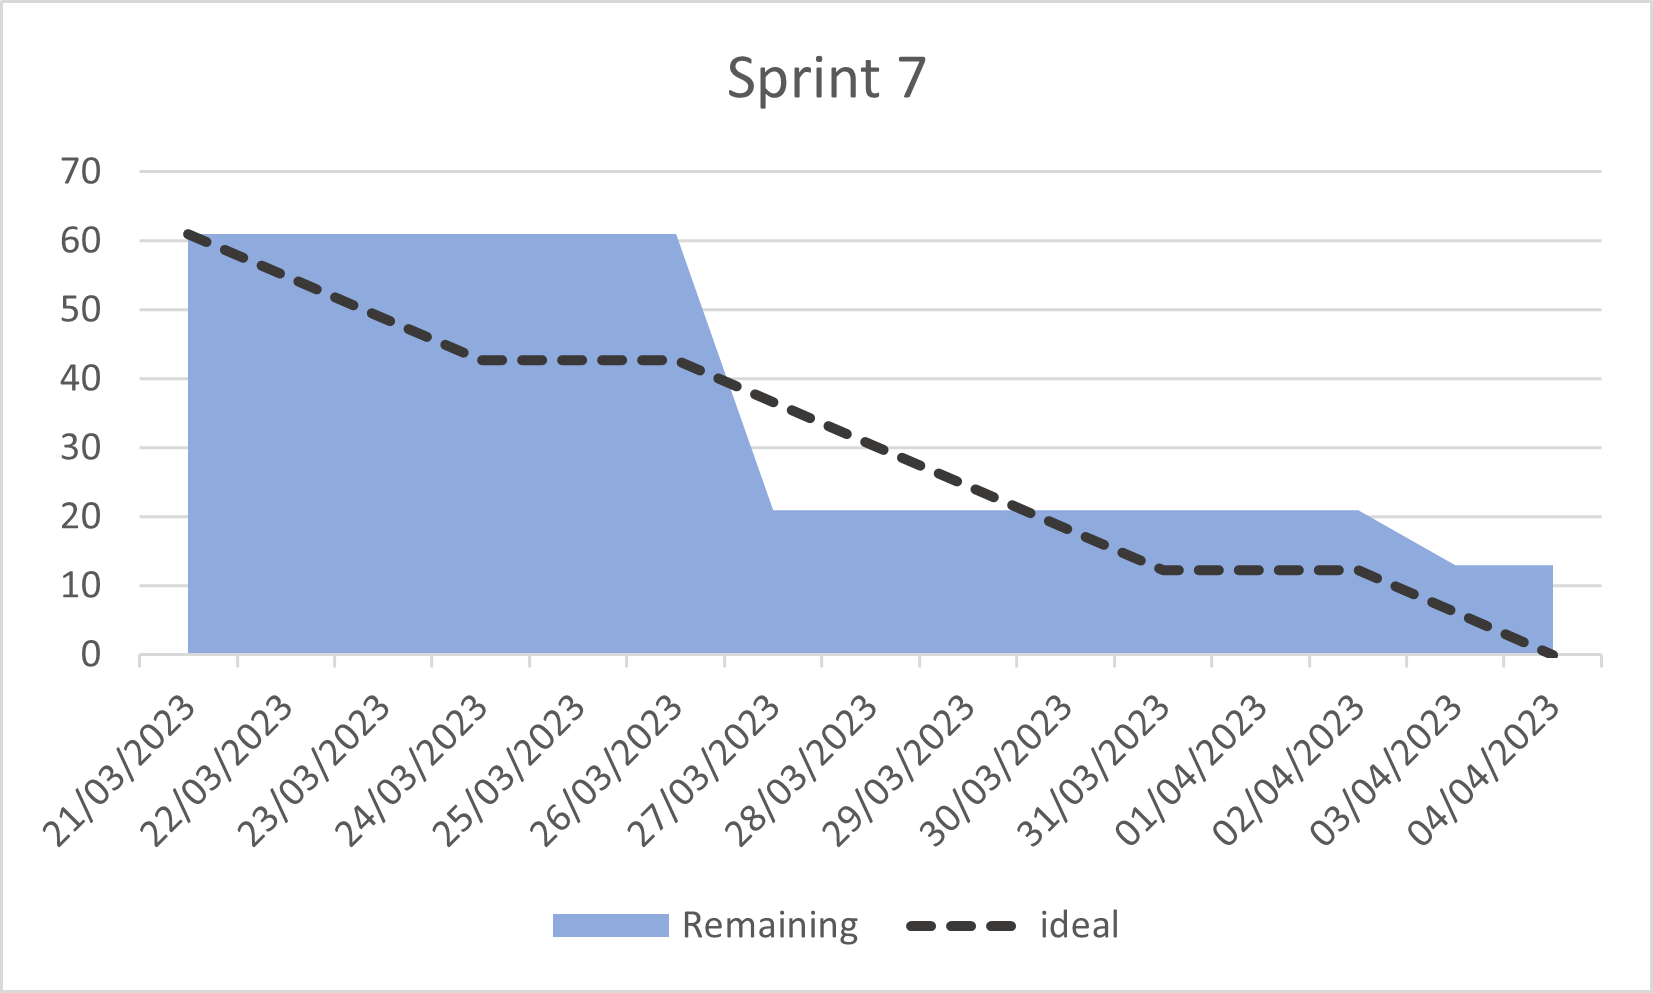
\includegraphics[width=0.9\textwidth]{burndown/septimoSprint.png}
         \caption{Sprint 7}
         \label{fig:Sprint7}
\end{figure}


\subsection{Sprint 8 - 04/04/2023 - 18/04/2023}

En el octavo sprint, planeó implementar la red neuronal convolucional VGG-16 para ir probando la implementación de Tensorflow Lite en Android Studio, además se programó  una tarea para comentar y refactorizar el código, esta tarea se planificó como si tuviera mucha dificultad, puesto que se era bastante código, pero finalmente, no fue tan laboriosa. Estas tareas se implementaron correctamente pudiendo terminar el sprint antes de tiempo. \ref{fig:Sprint8}
\begin{figure}[!ht]
         \centering
         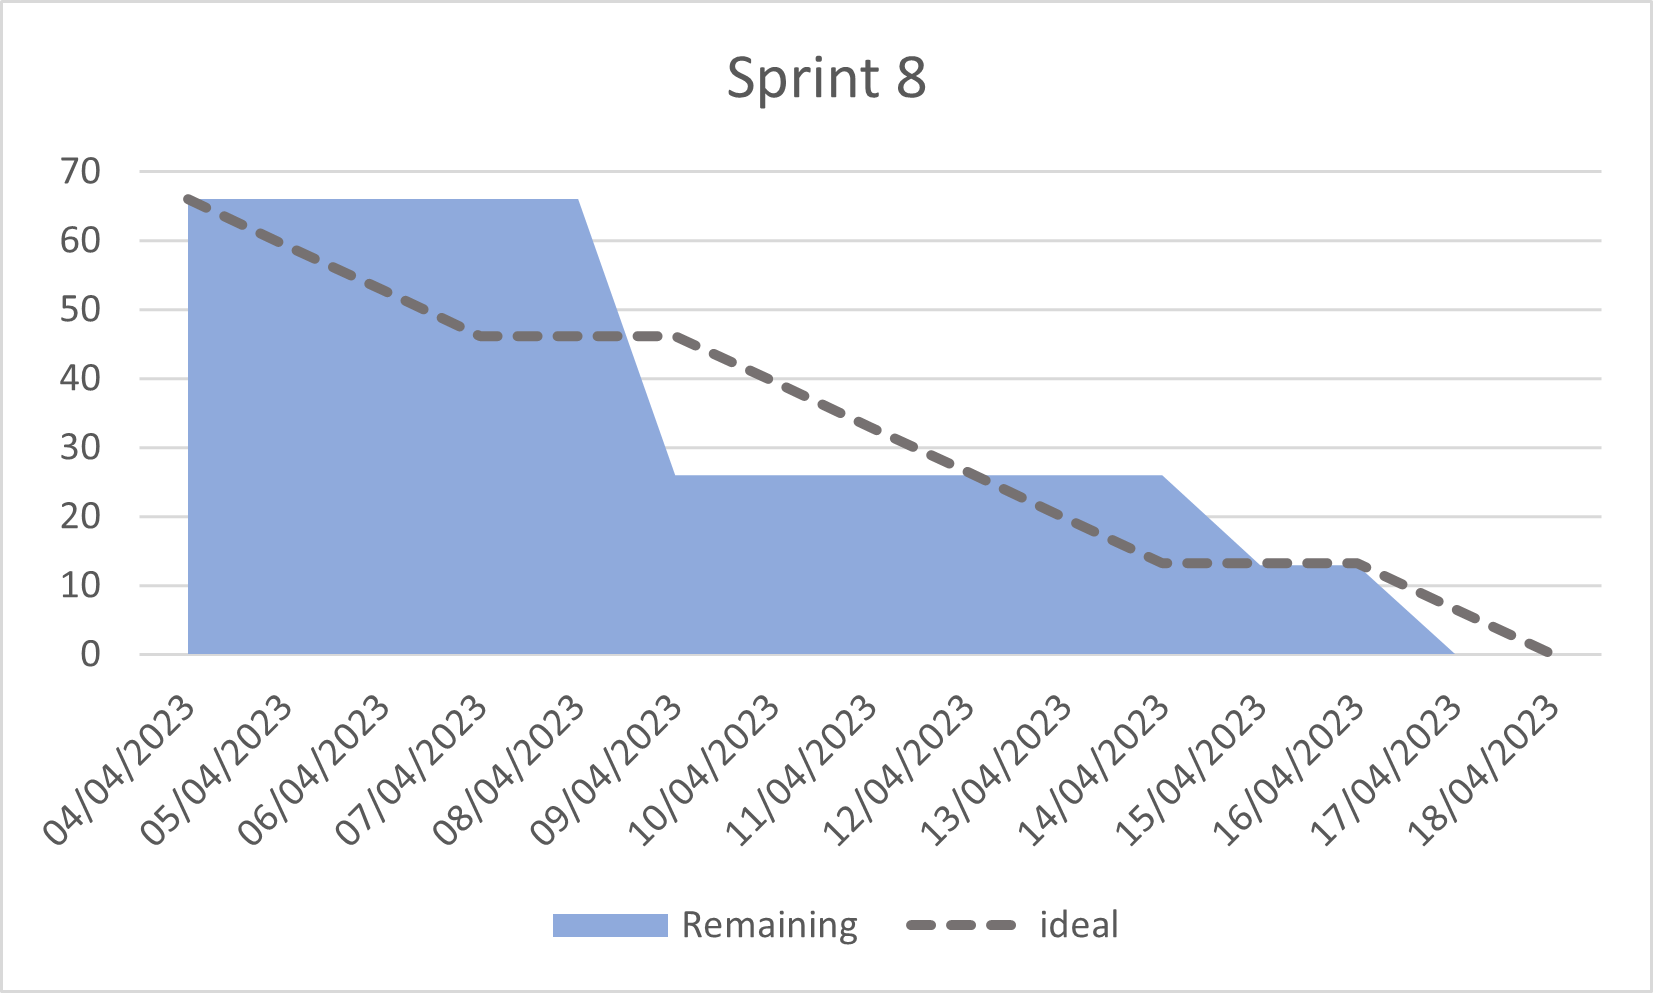
\includegraphics[width=0.9\textwidth]{burndown/octavoSprint.png}
         \caption{Sprint 8}
         \label{fig:Sprint8}
\end{figure}

\subsection{Sprint 9 - 18/04/2023 - 02/05/2023}
El noveno sprint se complicó el trabajo, puesto que se tenían que realizar varios exámenes y trabajos, teniendo así, un sprint con menos trabajo. Por lo que se planeó cambiar la base de datos a una consistente, de forma que los datos fueran persistentes entre sesiones, y seguir avanzando en el documento LaTeX, en concreto la introducción del plan de proyecto.

Considerando lo anterior, en el \textit{burndown} \ref{fig:Sprint9}, se puede apreciar como la primera semana no se avanzó mucho. Aun así, se consiguió terminar apuradamente las tareas del sprint.
\begin{figure}[!ht]
         \centering
         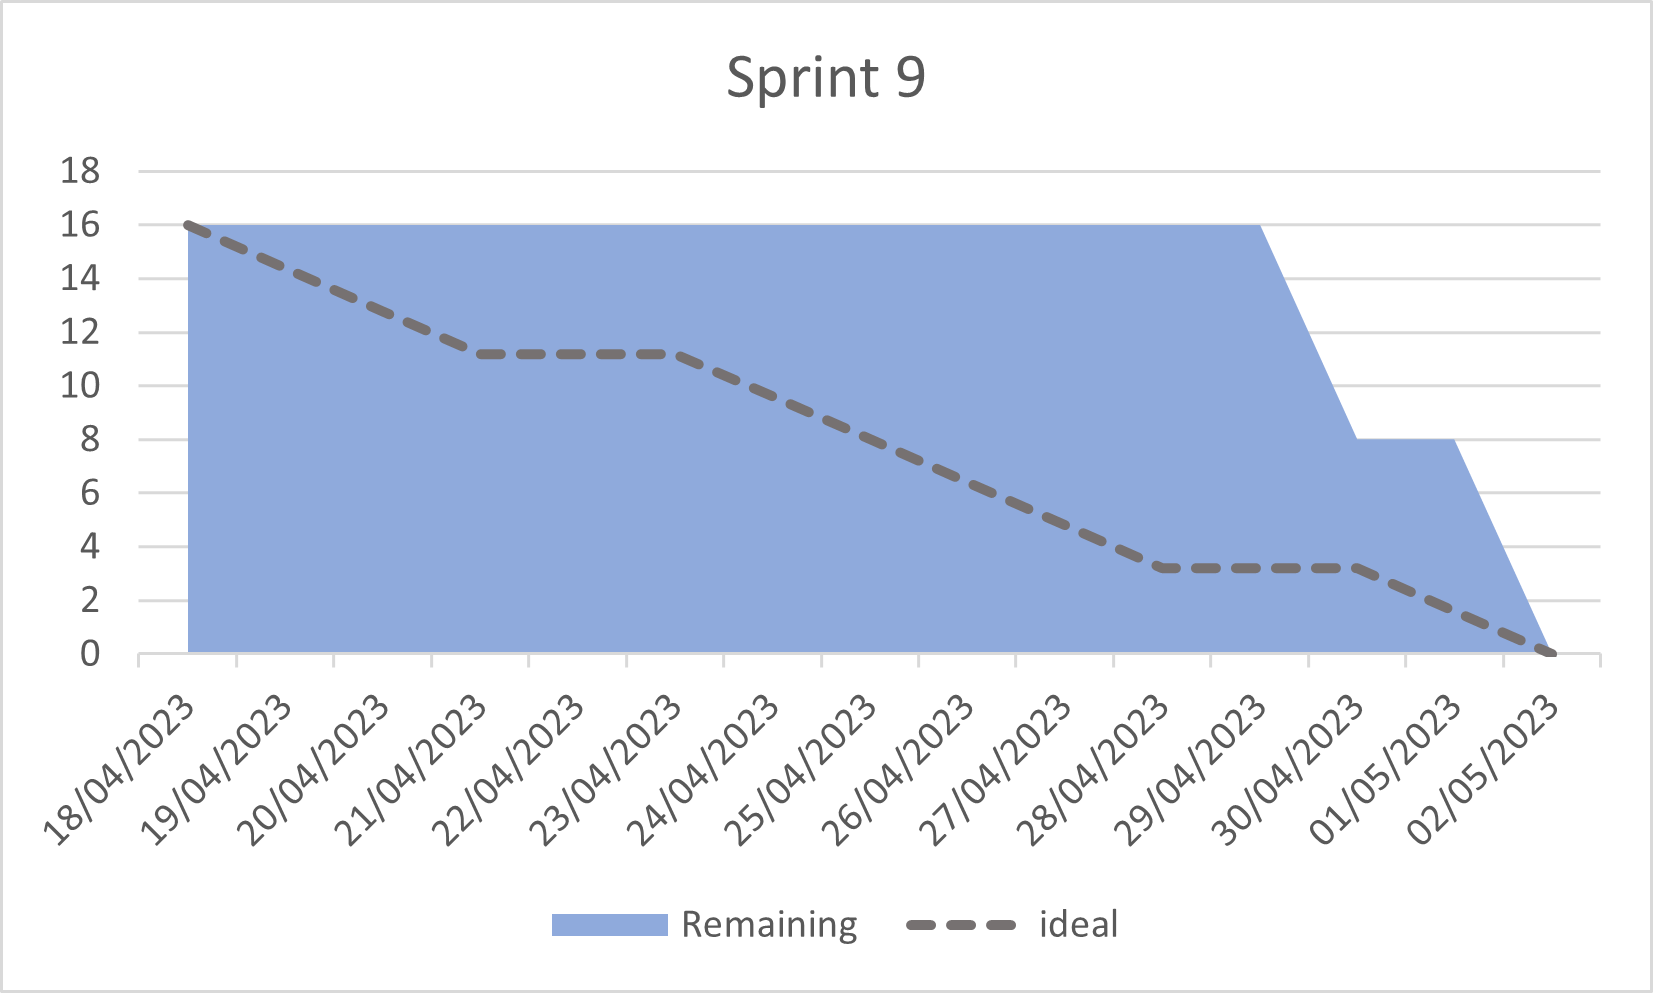
\includegraphics[width=0.9\textwidth]{burndown/novenoSprint.png}
         \caption{Sprint 9}
         \label{fig:Sprint9}
\end{figure}

\subsection{Sprint 10 - 02/05/2023 - 16/05/2023}

Al inicio de este sprint, se decidió no hacer desarrollo continuo con respecto al documento LaTeX, puesto que era complicado determinar cuándo hacer los commits, haciendo un commit al final del sprint con todo el cambio realizado. Además, se volvió a planear una eliminación de bugs y comentar el código, puesto que se habían ido haciendo pequeños cambios.

Al terminar el sprint se terminó el apartado ``Plan de proyecto'' aunque este se tendría que completar más adelante. \ref{fig:Sprint10}
\begin{figure}[!ht]
         \centering
         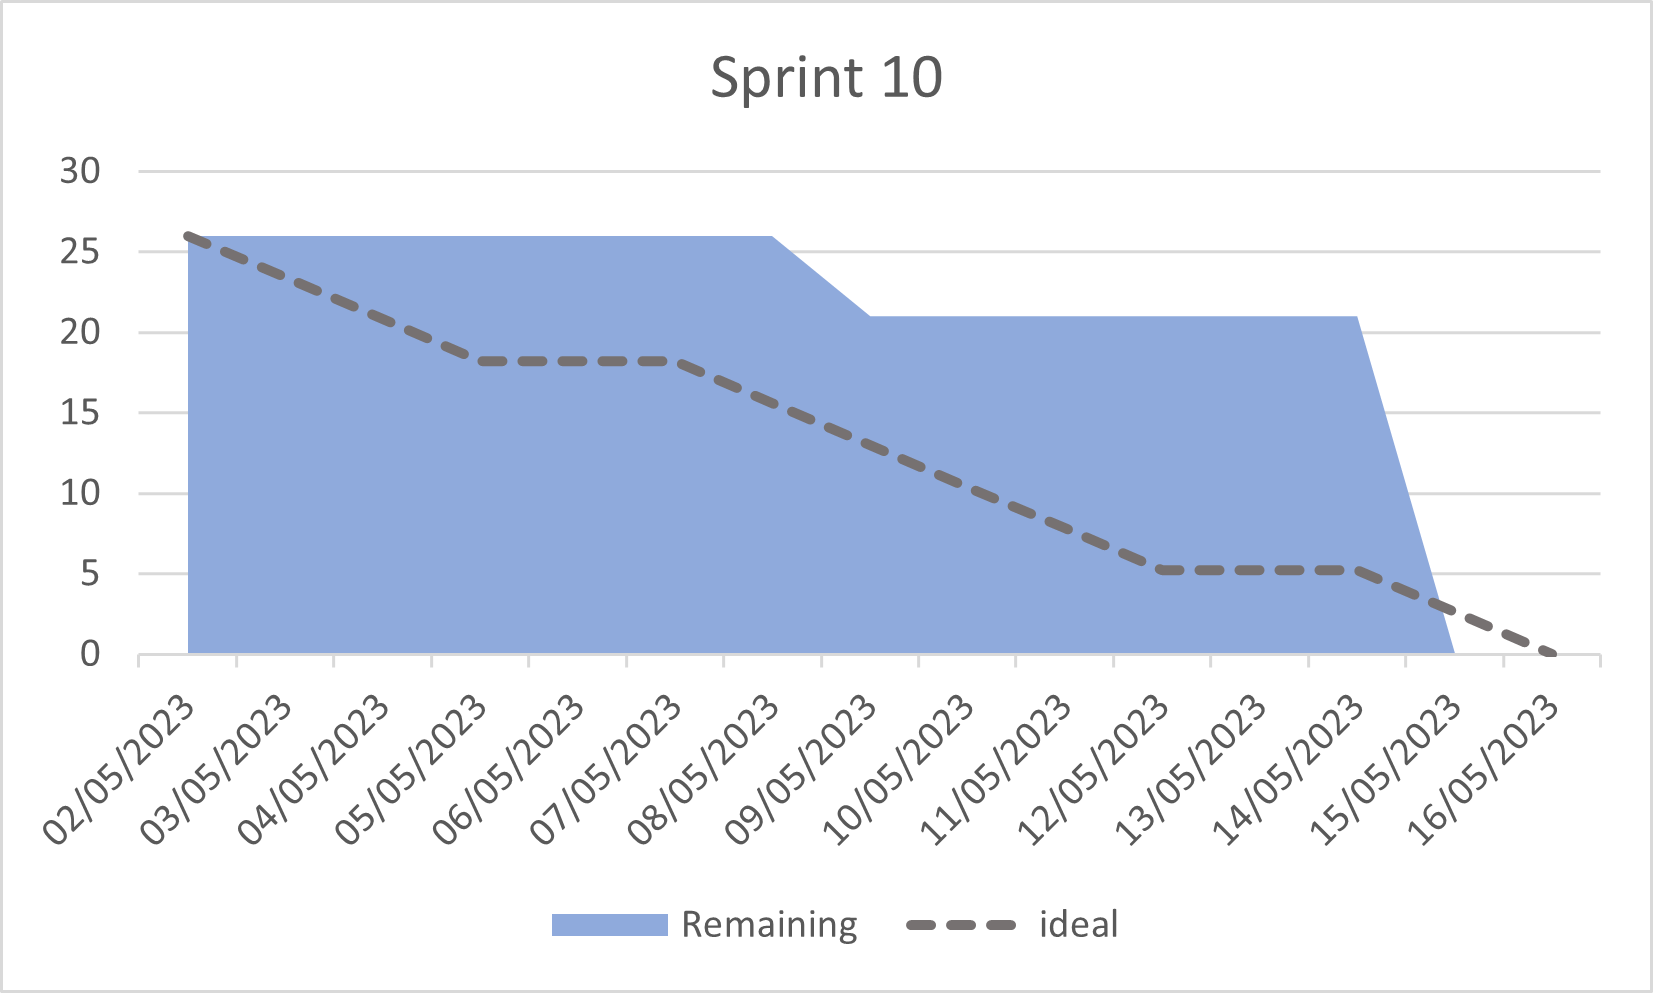
\includegraphics[width=0.9\textwidth]{burndown/decimoSprint.png}
         \caption{Sprint 10}
         \label{fig:Sprint10}
\end{figure}

\subsection{Sprint 11 - 16/05/2023 - 30/05/2023}
En este sprint, se obtuvo la primera red neuronal, planeando la tarea para este sprint. Además, se proporcionaron las imágenes, cada una con su respectiva calidad, pudiendo hacer una red neuronal convolucional con la que predecir si una foto tenía una calidad aceptable o no. Y como tarea continua, se siguió realizando el documento LaTeX. \ref{fig:Sprint11}

\begin{figure}[!ht]
         \centering
         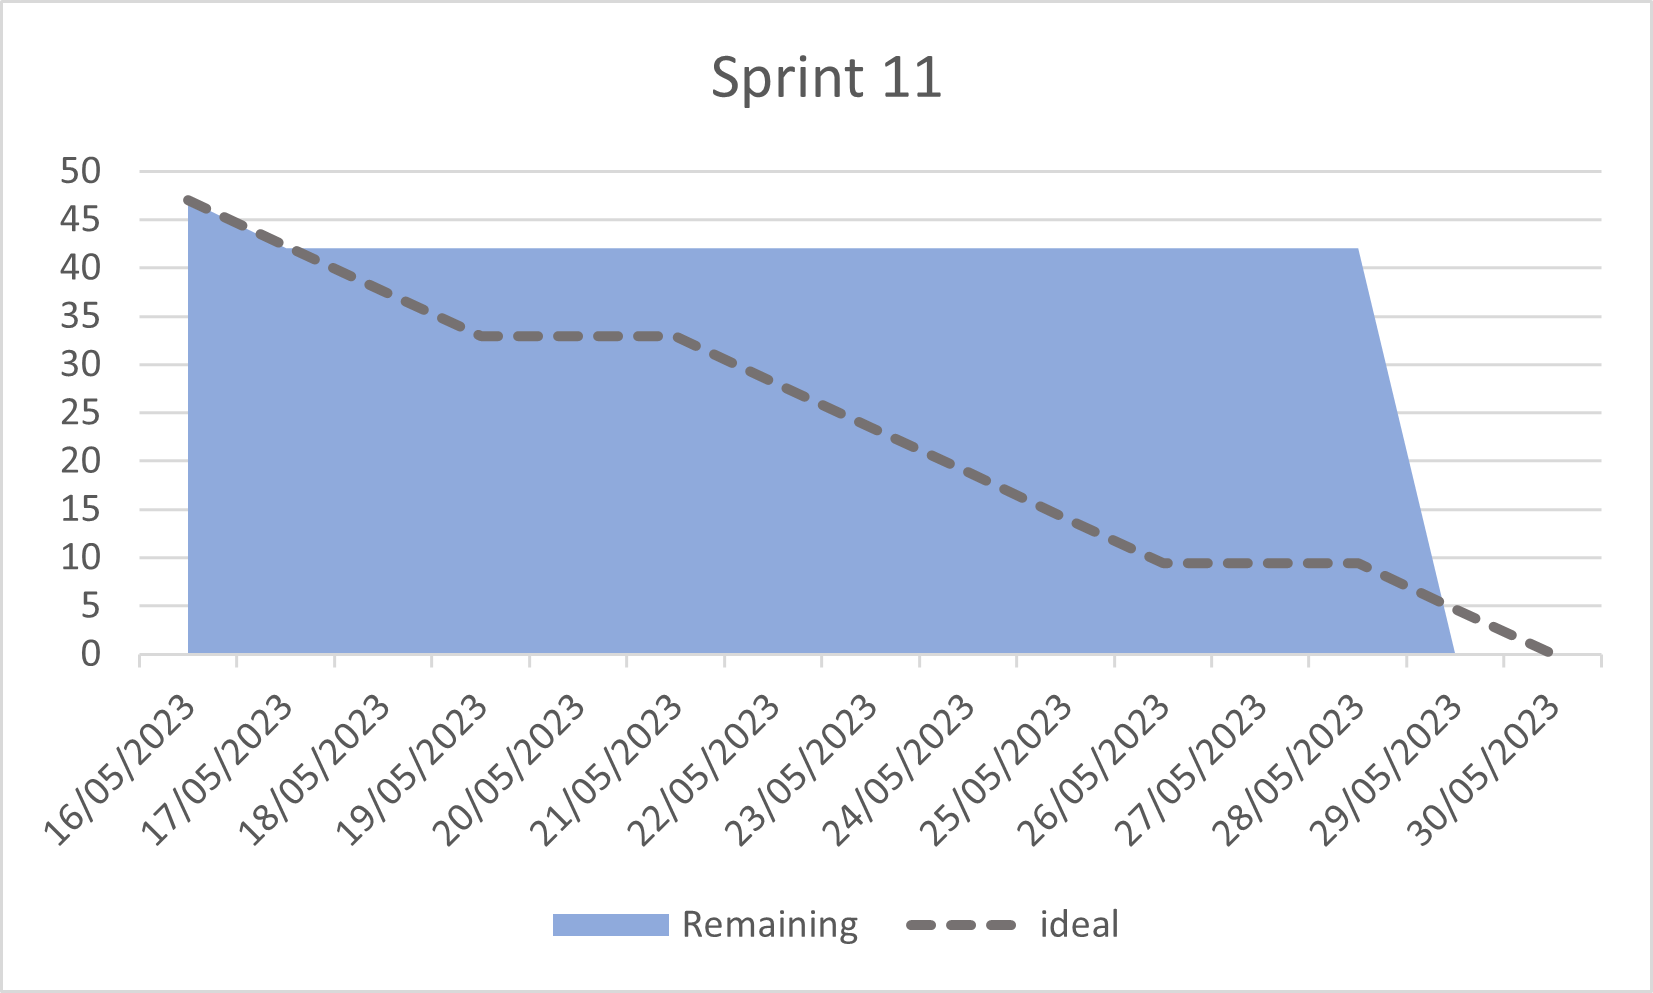
\includegraphics[width=0.9\textwidth]{burndown/decimoprimerSprint.png}
         \caption{Sprint 11}
         \label{fig:Sprint11}
\end{figure}
\subsection{Sprint 12 - 30/05/2023 - 13/06/2023}

Al iniciar el sprint, se descubrió que el conjunto de datos tenía desbalanceo, y, por tanto, la ``accuracy'' no era una métrica correcta para su uso. Por ese motivo, se decidió planear otra vez la tarea, cambiando las métricas. Y se siguió con el fichero LaTeX.
\ref{fig:Sprint12}
\begin{figure}[!ht]
         \centering
         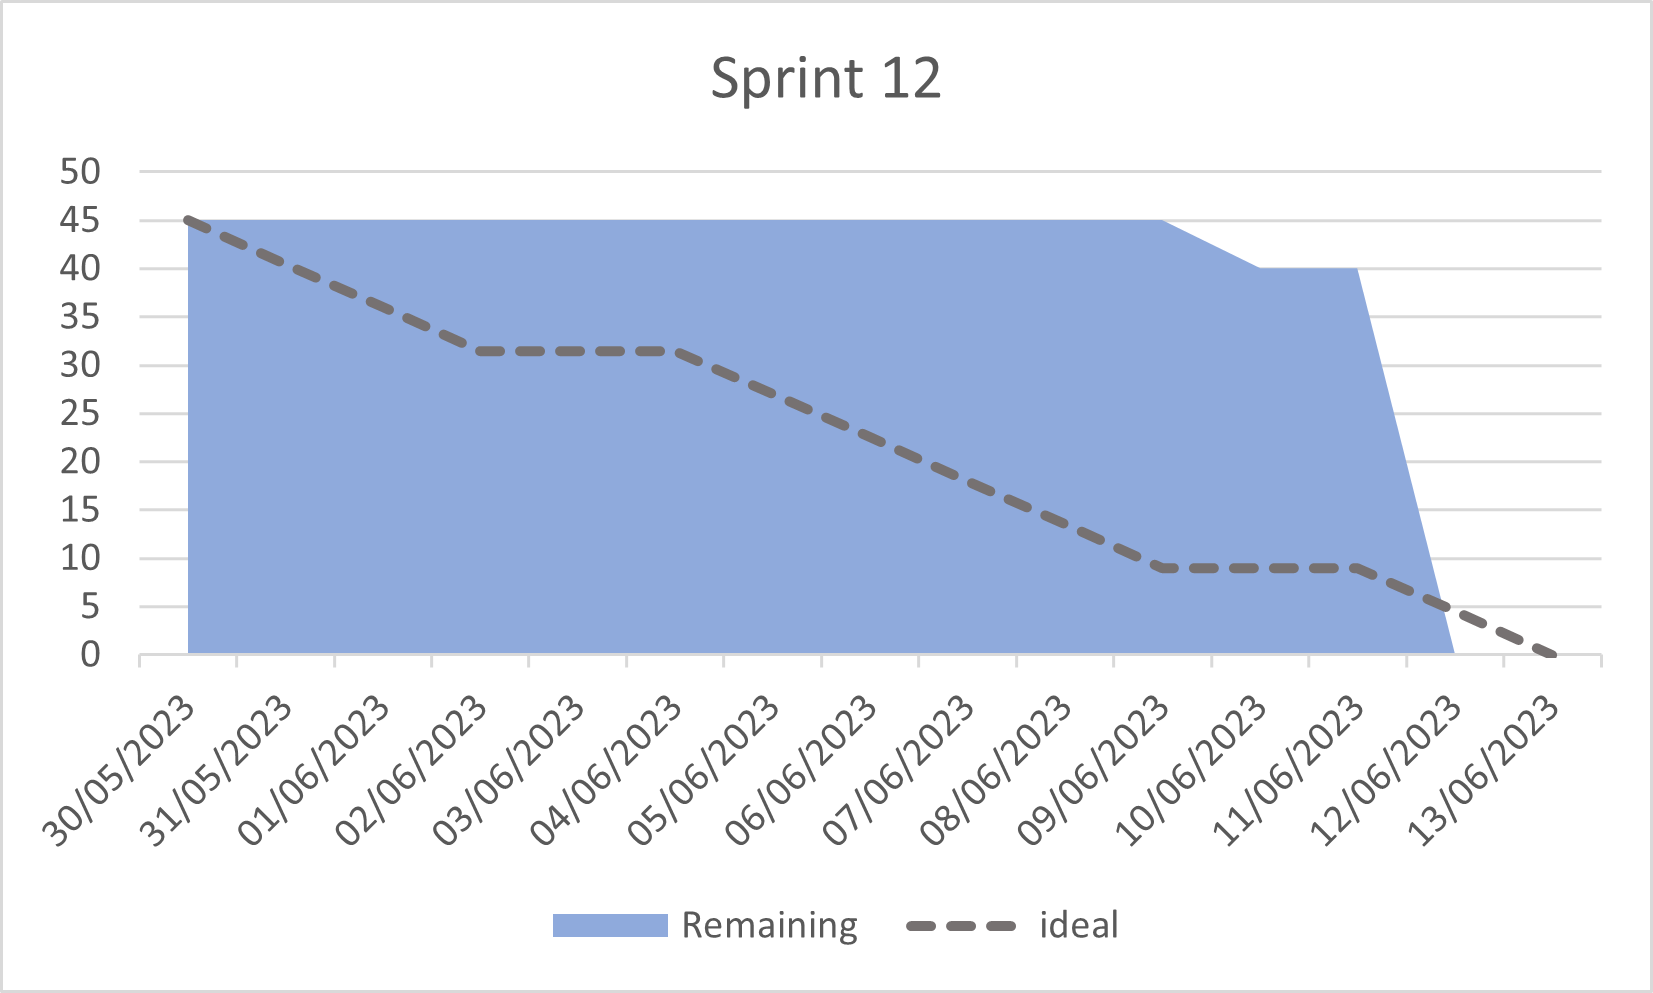
\includegraphics[width=0.9\textwidth]{burndown/decimosegundoSprint.png}
         \caption{Sprint 12}
         \label{fig:Sprint12}
\end{figure}

\subsection{Sprint 13 - 13/06/2023 - 27/06/2023}

En este sprint se terminó el documento LaTeX, y haciendo los retoques finales al proyecto para dejarlo entregable.
\ref{fig:Sprint13}
\begin{figure}[!ht]
         \centering
         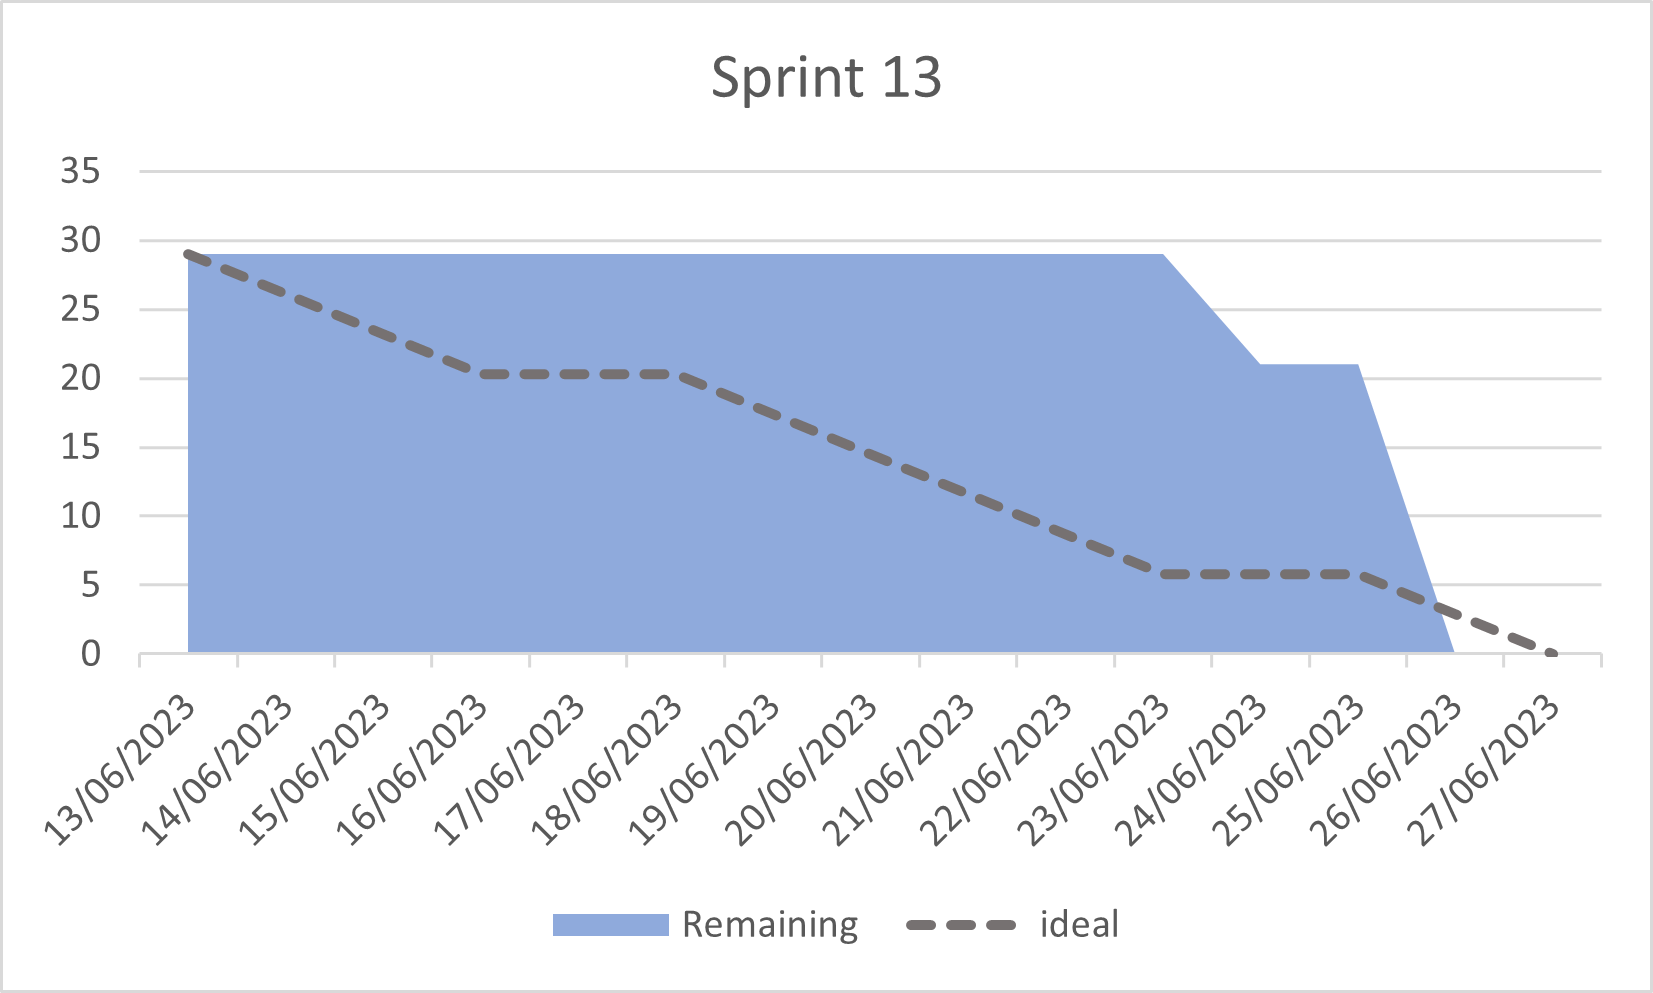
\includegraphics[width=0.9\textwidth]{burndown/decimotercerSprint.png}
         \caption{Sprint 13}
         \label{fig:Sprint13}
\end{figure}
\subsection{Sprint 14 - 27/06/2023 - 11/07/2023}

En este último sprint, se completó el documento LaTeX modificando partes para una mejor comprensión del texto.
\ref{fig:Sprint14}
\begin{figure}[!ht]
         \centering
         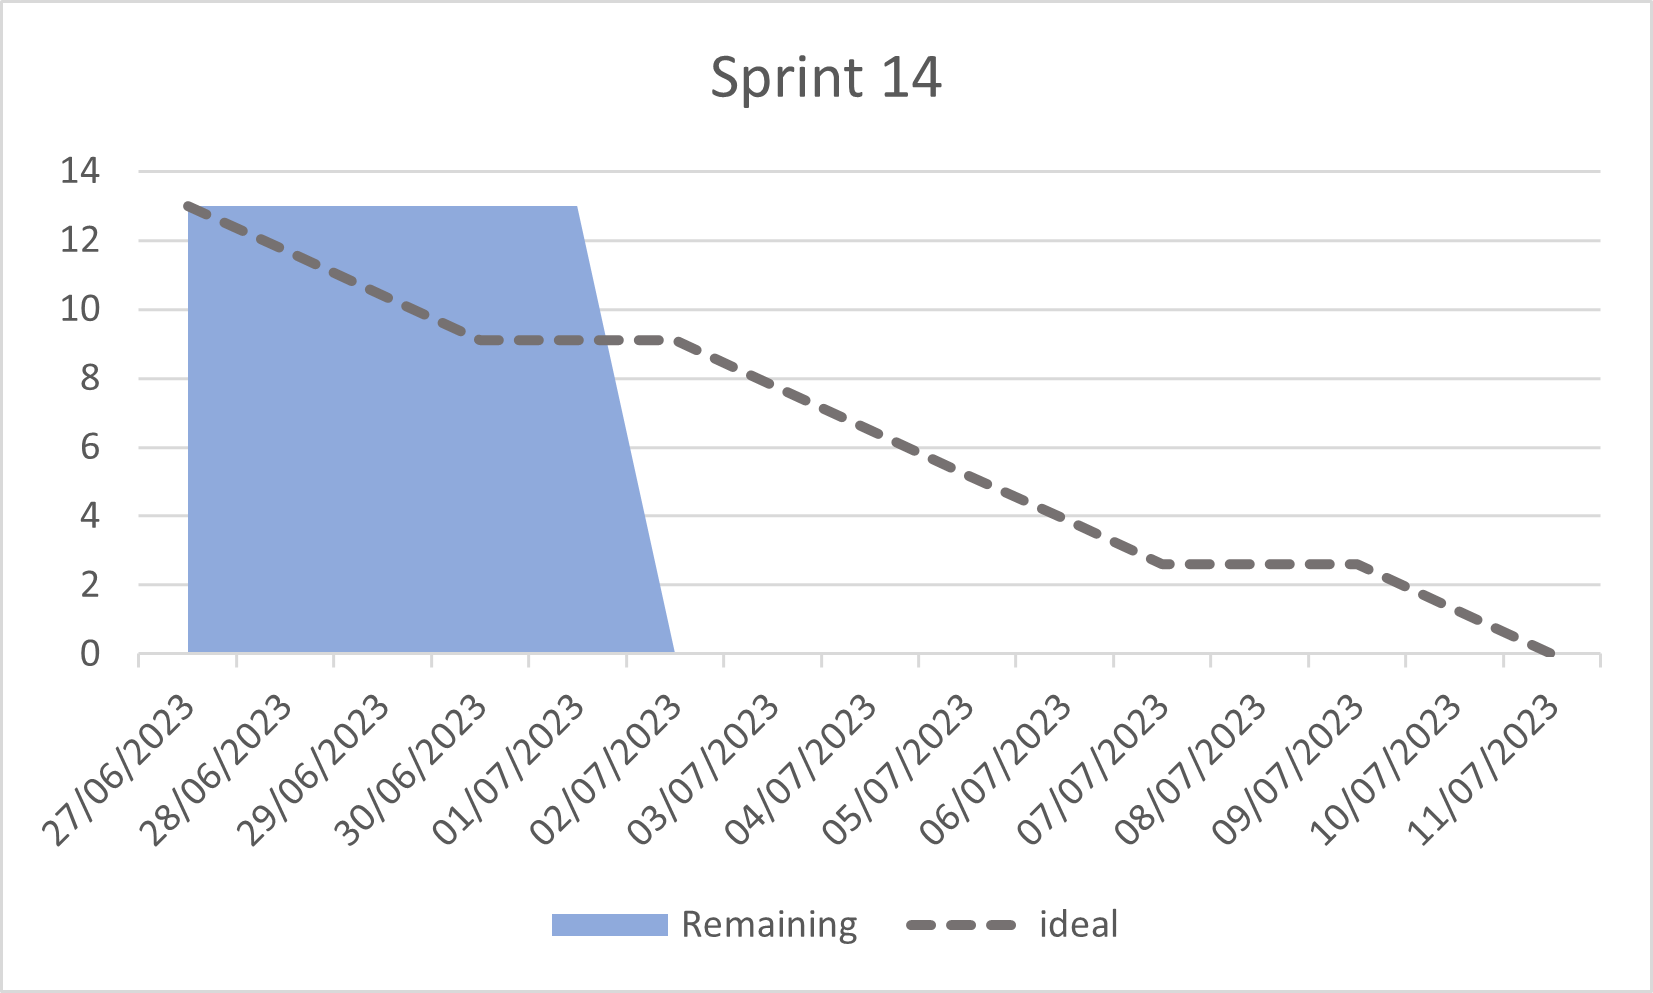
\includegraphics[width=0.9\textwidth]{burndown/decimocuartoSprint.png}
         \caption{Sprint 14}
         \label{fig:Sprint14}
\end{figure}

\section{Estudio de viabilidad}
Este proyecto, al estar orientado a la sanidad pública, no busca obtener beneficios, sino a facilitar la labor del médico.

En caso de querer desarrollar este proyecto con una intención comercial se muestra a continuación el estudio de viabilidad.

\subsection{Viabilidad económica}
\textbf{Costes}

\textbf{En personal}

Para el desarrollo del proyecto, se ha habría contratado a un programador \textit{junior} a tiempo parcial durante siete meses. 
Para la cotización de la seguridad social, se consideran los siguientes porcentajes:  un 23,60\% debido a las contingencias comunes, debido al desempleo de tipo general, al ser un contrato de tiempo indefinido, es un 5,50\%; un 0,2\% para el Fondo de Garantía Salarial, y un 0,60\% para formación profesional. Sumando estos porcentajes, un 29,9\% de retribución a la seguridad social.

\tablaSmall{Costes de personal}{l  c} {costesDePersonal}{Concepto & Coste\\} 
    {			Salario mensual neto & 973\euro\\
                Tipo de retención del IRPF & 11.69\%\\
			Cuota a pagar del IRPF  & 195\euro\\
			Seguridad Social (29.9\%)& 498\euro\\
			Salario mensual bruto & 1.666\euro\\
			\hline
			\textbf{Total 6 meses} & 9.996\euro\\}

El coste se puede ver en la tabla: \ref{tabla:costesDePersonal}

\textbf{En \textit{hardware}}

Para realizar el proyecto, se hará uso de un ordenador portátil y opcionalmente, un dispositivo móvil, para comprobar el correcto funcionamiento de la aplicación.

Suponiendo que los dispositivos hardware se amortizan en seis años, y se han utilizado durante siete meses:

\tablaSmall{Costes de Hardware}{l  cc} {costesDeHardware}{Concepto & Coste & Amortización\\} 
    {			Ordenador & 1.200\euro & 100\euro\\
                Dispositivo móvil & 300 \euro & 25\euro\\
                Oftalmoscopio Portátil D-Eye & 400\euro & 33,33\euro \\
			\hline
			\textbf{Total} & 1.900\euro & 158,33\euro\\}

El coste se puede ver en la tabla: \ref{tabla:costesDeHardware}

\textbf{En \textit{software}}

Se muestran aquellas licencias de \textit{software} que no son gratuitas, y considerando que su amortización es de un año.
\tablaSmall{Costes de Software}{l  cc} {costesDeSoftware}{Concepto & Coste & Amortización\\} 
    {			Windows 11 Pro & 259\euro & 129,5\euro\\
                ZenHub para equipos (3 meses) & 36\euro & 18 \euro\\
			\hline
			\textbf{Total} & 295\euro & 147,5\euro\\}

El coste se puede ver en la tabla: \ref{tabla:costesDeSoftware}
   
\textbf{Costes adicionales}

Como se pretende comercializar la aplicación, la \textit{Play Store} es una de las mejores plataformas de distribución de aplicaciones móviles. Pero, para publicar una aplicación, es necesario una cuenta de desarrollador, la cual cuesta 25€.
\tablaSmall{Costes adicionales}{l  c} {costesAdicionales}{Concepto & Coste\\} 
    {			Cuenta de desarrollador Play Store & 25\euro\\
                Internet & 210\euro \\
                Alquiler de oficina & 800\euro \\
			\hline
			\textbf{Total} & 1.035\euro \\}

   El coste se puede ver en la tabla: \ref{tabla:costesAdicionales}

\textbf{Costes totales}

Siendo los costes totales, los vistos en: \ref{tabla:costesTotales}
\tablaSmall{Costes totales}{l  c} {costesTotales}{Concepto & Coste\\} 
    {			En personal & 9.996\euro\\
                En hardware & 1.900\euro \\
                En software & 295\euro \\
                Adicionales & 1.035\euro \\
			\hline
			\textbf{Total} & 13.226\euro \\}

\textbf{Beneficios}

Como se ha comentado anteriormente, el proyecto tiene un objetivo altruista de ayudar en la labor del médico, dejando a un lado el objetivo de lucrarse con el proyecto. Hay varios focos en los que se podrían obtener beneficios:
\begin{itemize}
    \item Vender la aplicación al servicio sanitario, con un beneficio del 30\%. Dando la opción de comprar servicios de mantenimiento.
    \item Ofrecer licencias de la aplicación, cobrando cada año por mantener la suscripción.
    \item Introducir anuncios en la aplicación.
    \item Distintas licencias de la aplicación, cada una con unas ventajas, con diferentes precios.
\end{itemize}

Entre las opciones anteriores, se ha descartado el uso de anuncios, principalmente, porque elimina profesionalidad a la aplicación; y también la opción de las distintas licencias, pero al ofrecer un único servicio, no se podía plantear esta opción.

Como las otras dos opciones se han considerado viables, se desarrollarán a continuación, además, es importante recalcar que los valores pueden  cambiar debido a la gran cantidad de centro sanitarios públicos que hay, proporcionando ofertas según esa cantidad.

\textbf{Vender la aplicación}

Vendiendo la aplicación al servicio sanitario, solo se realizaría un pago por la compra, de forma que la empresa obtenga un 30\% de beneficios.
De esta forma, 13.226\euro  sería el 70\% del precio y la aplicación se vendería por 18.894,28\euro; dando un beneficio de 5.668,28 \euro. 

También se podría ofrecer al servicio sanitario una opción de compra, donde la empresa se encarga de hacer el mantenimiento y actualizaciones de la aplicación. Siendo un servicio que depende del numero de centros sanitarios que haya en la comunidad autónoma. Un posible precio razonable, sería que, por cada centro sanitario, anualmente se pague una tarifa de 10\euro. 

Poniendo el caso de que el SACYL comprase la aplicación para el 25\% de los centros sanitarios, como tiene 10.218,
debería pagar por (10.218 * 0,25 * 10 ), siendo de esta forma anualmente se alcanzaría una cifra de 25.545\euro  al año.
Como una persona cuesta cada 6 meses, 9.996\euro, al año serian 19.992\euro, teniendo beneficios anuales.


\textbf{Licencias de la aplicación}

Como el caso anterior, se va a hacer una oferta por cada centro sanitario, donde anualmente, se cobraría 100\euro.

Suponiendo que el SACYL pidiese una licencia para todos los centros, se haría el cálculo de $(10.218 * 0,25 * 100 ) $ dando una cifra anual de 255.450\euro  en este precio ya estaría incluido el precio del mantenimiento.

En este caso, la empresa se encargaría de ofrecer los servicios al SACYL, se debería contratar un servidor con una base de datos, como el servidor guarda imágenes, se necesitaría bastante espacio, pongamos que se contrata un servidor Microsoft SQL Server de 1 GB, con un precio de 350\euro  al mes. Como 1GB pueden ser poco para Castilla y León, se considera que se compran 50 servidores. Añadiendo al coste anual, $4200 * 50 $ siendo así, 210.000\euro

Por tanto, con 255.450 \euro  al año; habría que restar el coste de los servidores y el del personal donde se podría aumentar el número a 2 personas,   255.450 - 210.000 - 39.984 , haciendo que anualmente, se tengan 5.466 \euro   de beneficio, como el coste de la aplicación era de 13.226 \euro, harían falta 3 años para obtener un beneficio real sobre el proyecto.

\textbf{Otros casos}

Hay un caso que es importante destacar, y es el caso concreto de que el SACYL fuese la empresa encargada.

En este caso, no hay ningún beneficio monetario para la empresa, puesto que es sanidad pública. Pero, realizando el proyecto, a futuro se pueden evitar costes adicionales, como, por ejemplo: 
\begin{itemize}
    \item Coste de transporte de la ambulancia.
    \item Costes de citas innecesarias y el tiempo que conllevan estas.
    \item Costes de material utilizado.
\end{itemize}

\subsection{Viabilidad legal}

\textbf{Software}

Esta sección aborda el contexto legal del proyecto, junto con las licencias \textit{software} utilizadas.
\tabla{Dependencias del proyecto Android}{|p{2.5cm}|c|p{5cm}|p{3.5cm}|}{4}{dependenciasAndroid}{Dependencia & Versión & Descripción & Licencia\\}{
Appcompat & 1.6.1 & Permite a versiones anteriores de Android una compatibilidad mejorada & Apache License 2.0\\
Material  & 1.8.0 & Proporciona componentes de Material Design para Android. & Apache License 2.0\\
Constraint Layout & 2.1.4 & Permite crear diseños complejos y flexibles & Apache License 2.0 \\
JUnit & 4.13.2 & Framework de pruebas unitarias en Java & Eclipse Public License 1.0\\
Ext JUnit & 1.1.5 & Biblioteca de pruebas unitarias para Android que extiende JUnit & Apache License 2.0\\
Espresso-core & 3.5.1 & Biblioteca de pruebas de interfaz de usuario & Apache License 2.0 \\
TensorFlow Lite & 2.7.0 & Biblioteca de aprendizaje automático, más ligera que TensorFlow & Apache License 2.0 \\
SQLite & 2.2.0 & Biblioteca que utiliza bases de datos SQLite, proporcionando una API para interactuar con la base de datos & No requiere\\
}
\newpage
Como el proyecto también ha tenido una parte realizada en Python, se incluyen las dependencias utilizadas.
\tabla{Dependencias del proyecto Python}{|p{2.5cm}|c|p{5cm}|p{3.5cm}|}{4}{dependenciasPython}{Dependencia & Versión & Descripción & Licencia\\}{
sys & 3.10.8 & Módulo de la librería estándar de Python que permite trabajar con tiempos & Python Software Foundation \\
NumPy  & 1.23.5 & Permite manejar \textit{arrays}, álgebra lineal, transformaciones de fourier y matrices & BSD 3-Clause \\
Pandas & 2.0.1 & Permite analizar, limpiar, explorar y manipular el conjuntos de datos. & BSD 3-Clause  \\
matplotlib & 3.6.2 & Permite ver visualmente gráficas de nivel bajo & Python Software Foundation \\
scikit-learn & 1.2.2 & Es un modulo para aprendizaje automático. & BSD 3-Clause \\
TensorFlow & 2.14.0 & Biblioteca de aprendizaje automático & Apache License 2.0 \\
}

\textbf{Imágenes}

Hay varios tipos de imágenes utilizadas en el proyecto, donde el logo, se ha utilizado usando DALLE2, la cual en sus políticas y términos se explica que el usuario tiene todos los derechos, tanto comerciales y no comerciales.

Por otro lado, para los iconos de la aplicación, se usaron tanto iconos por defecto de Android Studio, como iconos de Google Fonts, donde todas las imágenes son de código abierto y no tienen costo. Con una licencia Apache 2.0.




\textbf{Licencia del proyecto}

En resumen, el proyecto utiliza varios tipos de licencias que son por orden de más permisivas a menos:  BSD 3-Clause License, Python Software Foundation License, Apache License 2.0 y Eclipse Public License 1.0.

Una licencia que se adapta a las condiciones buscadas es GNU General Public License v3. En la imagen \ref{fig:Licencia GPLv3} se puede observar correctamente las características que ofrece.
\begin{figure}[!ht]
         \centering
         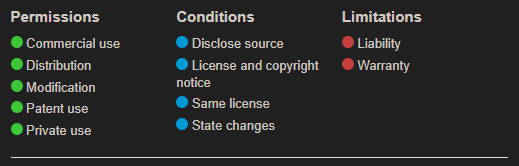
\includegraphics[width=0.9\textwidth]{img/GPLv3.png}
         \caption{Licencia GPLv3. Imagen obtenida de \url{https://choosealicense.com/licenses/}}
         \label{fig:Licencia GPLv3}
\end{figure}

Al comprobar la compatibilidad de las licencias con la GNU, se comprobó que Eclipse Public License 1.0 no es compatible con esta.
En este caso, se opto por utilizar una doble licencia EPL y Apache License 2.0; donde EPL afectaría solo a los test unitarios y la demás parte del proyecto sería liberada con Apache License 2.0.



\subsection{Marco legal del proyecto}

Es importante recalcar que al estar trabajando sobre una aplicación que usa datos delicados de las personas, siendo estos, además, datos relacionados con la salud. 

\textbf{RGPD}

Según viene descrito en el artículo 9 del Reglamento General de Protección de Datos, está prohibido hacer un tratamiento de categorías especiales de datos personales a menos que ocurra:
\begin{itemize}
    \item El interesado ha dado el consentimiento explicito para el tratamiento de datos.
    \item Resulte necesario para proteger los intereses vitales del interesado u otra persona física cuando no este capacitado para dar su consentimiento.
    \item Es necesario para fines de medicina preventiva o laboral.
    \item Es necesario con fines de archivo en interés público, fines de investigación científica o histórica o fines estadísticos.
\end{itemize}

En el \href{https://www.boe.es/doue/2016/119/L00001-00088.pdf#page=38}{artículo 9}, vienen más puntos, pero solo se explican los referentes al uso de la aplicación.

En el \href{https://www.boe.es/doue/2016/119/L00001-00088.pdf#page=47}{capítulo 4} del Reglamento General de Protección de Datos, se trata sobre el responsable de  tratar los datos y  el encargado del tratamiento.

Por ello, con el fin de evitar que los datos sensibles se confundan entre los distintos pacientes, se ha implementado una interfaz, en la cual el médico introduce el DNI del paciente a ser tratado en ese momento, mostrando el nombre del paciente del DNI, en caso de haberse confundido a la hora de poner el DNI, se podrá dar cuenta al ver el nombre del paciente. 
